% ======================================================================
% Relatório de Desenvolvimento do Projeto compass_sim — V01
% Gerado em 04/07/2026. Histórico coberto: 15/06/2026 a 04/07/2026.
% Compilar com: pdflatex relatorio_projeto_V01.tex (2x para referências)
% ======================================================================
\documentclass[11pt,a4paper]{article}

\usepackage[utf8]{inputenc}
\usepackage[T1]{fontenc}
\usepackage[brazilian]{babel}
\usepackage{geometry}
\geometry{margin=2.5cm}
\usepackage{graphicx}
\usepackage{booktabs}
\usepackage{longtable}
\usepackage{amsmath}
\usepackage{amssymb}
\usepackage{siunitx}
\usepackage{hyperref}
\usepackage{xcolor}
\hypersetup{colorlinks=true, linkcolor=blue!50!black, urlcolor=blue!50!black,
            citecolor=blue!50!black}
\usepackage{caption}
\captionsetup{font=small, labelfont=bf}

\newcommand{\code}[1]{\texttt{#1}}

\title{\textbf{Simulação de redes de agulhas magnéticas dipolares:\\
relatório de desenvolvimento do projeto \code{compass\_sim}}\\[1ex]
\large Versão V10 do relatório}
\author{J.~P.~Sinnecker}
\date{4 de julho de 2026\\[0.5ex]
\small Período coberto: 15/06/2026 -- 04/07/2026}

\begin{document}
\maketitle

\begin{abstract}
\noindent
Este relatório documenta o desenvolvimento completo do projeto
\code{compass\_sim}: um simulador em Python de redes bidimensionais de
agulhas de bússola magnéticas interagindo por acoplamento dipolar
completo, com dinâmica newtoniana inercial em unidades do SI. O projeto
nasceu como demonstração pedagógica da analogia entre arranjos de
bússolas e materiais magnéticos (histerese, formação de domínios) e
evoluiu, ao longo de seis sessões de desenvolvimento, para um
instrumento de pesquisa com potencial de publicação. O relatório
registra, passo a passo, as decisões de projeto, os problemas
encontrados e suas soluções, o registro de versões do código
(V20--V39), a estratégia de pesquisa e publicação construída sobre uma
lacuna identificada na literatura, e os resultados do estudo-piloto da
campanha ``amortecimento~$\times$~histerese/avalanches'', que já exibe o
sinal central procurado: crescimento sistemático do expoente de
avalanche $\tau$ com o fator de qualidade $Q$.
\end{abstract}

\tableofcontents
\newpage

% ======================================================================
\section{Objetivo do projeto}
% ======================================================================

O projeto tem hoje dois objetivos em camadas, que refletem sua evolução
histórica:

\paragraph{Objetivo original (pedagógico/demonstrativo).}
Construir uma simulação visual de uma rede de agulhas de bússola que
giram exclusivamente sob o campo magnético que cada uma gera sobre as
vizinhas, buscando o equilíbrio coletivo de direções --- uma analogia
mecânica direta e intuitiva com materiais magnéticos reais, capaz de
exibir comportamento histerético e formação de domínios magnéticos,
vista de cima e exportável em vídeo.

\paragraph{Objetivo atual (científico).}
Usar o simulador --- que implementa dinâmica \emph{inercial} newtoniana
real, algo raro na literatura da área --- para responder a uma pergunta
de física estatística fora do equilíbrio com potencial de publicação:

\begin{quote}\itshape
O coeficiente de amortecimento controla a classe de universalidade das
avalanches e a forma do laço de histerese em redes dipolares clássicas
com acoplamento de longo alcance e anisotrópico? E essa resposta depende
da geometria da rede (quadrada, triangular, honeycomb), isto é, da
frustração geométrica?
\end{quote}

A literatura estabeleceu que sistemas subamortecidos e sobreamortecidos
pertencem a classes de universalidade distintas em modelos de curto
alcance ou de campo médio (Kuramoto com inércia, Ising com
amortecimento, sólidos amorfos cisalhados)~\cite{dahmen2011}. A lacuna
identificada: ninguém verificou se esse quadro sobrevive ao acoplamento
dipolar real --- de longo alcance ($\sim 1/r^3$) e anisotrópico --- em
redes bidimensionais com dinâmica angular contínua e inércia física. O
simulador deste projeto é, até onde a revisão de literatura alcançou, o
único instrumento montado especificamente para essa pergunta.

% ======================================================================
\section{O modelo físico}
% ======================================================================

Cada agulha $i$ é um dipolo magnético pontual de momento $m$ fixado em
uma posição $\vec r_i$ da rede, livre para girar no plano em torno de um
pino central sem atrito de contato, mas com amortecimento viscoso (ar).
A dinâmica é a segunda lei de Newton rotacional:
\begin{equation}
I\,\ddot\theta_i \;=\; \tau_i^{\mathrm{dip}} + \tau_i^{\mathrm{ext}}
- b\,\dot\theta_i,
\label{eq:eom}
\end{equation}
onde $I$ é o momento de inércia da agulha, $b$ o coeficiente de
amortecimento viscoso e os torques vêm de $\vec\tau = \vec m \times \vec
B$. O campo dipolar sobre a agulha $i$ soma as contribuições de
\emph{todas} as demais agulhas (acoplamento completo, custo
$\mathcal{O}(K^2)$ para $K$ agulhas):
\begin{equation}
\vec B_j(\vec r_i) = \frac{\mu_0}{4\pi}\,
\frac{3(\vec m_j \cdot \hat r)\hat r - \vec m_j}{r^3},
\qquad \vec r = \vec r_i - \vec r_j .
\end{equation}

A integração usa o esquema Velocity--Verlet com passo $\Delta t$
proporcional ao período natural $T_0 = 2\pi/\omega_0$, onde
\begin{equation}
\omega_0 = \sqrt{\frac{m\,B_{\mathrm{ref}}}{I}},
\qquad
B_{\mathrm{ref}} = \frac{\mu_0}{4\pi}\frac{2m}{r_{nn}^{3}}
\end{equation}
é a frequência de pequenas oscilações no campo dipolar de referência
entre primeiros vizinhos (separação $r_{nn}$). O regime dinâmico é
caracterizado pelo fator de qualidade
\begin{equation}
Q = \frac{\omega_0 I}{b},
\end{equation}
com $Q \gg 1$ subamortecido (oscilatório) e $Q \ll 1$ sobreamortecido
(relaxação monotônica). Esse é o parâmetro de controle central do estudo
científico.

\paragraph{Parâmetros físicos reais.}
Uma decisão estruturante do projeto foi usar unidades do SI e derivar os
parâmetros da geometria real da agulha, em vez de constantes arbitrárias:
\begin{itemize}
\item \textbf{Momento de inércia}: calculado para uma lâmina de aço de
\SI{0.4}{mm} de espessura com o formato de losango da agulha (por
exemplo, $I \approx \SI{3.8e-11}{kg.m^2}$ e massa $\approx$
\SI{0.017}{g} para agulha de \SI{0.5}{cm});
\item \textbf{Momento magnético}: assumindo o aço saturado ao longo do
eixo maior, $m = M_s V$, com $M_s = \SI{1.59e6}{A/m}$ (aço-carbono
comum, $B_{\mathrm{sat}} \approx \SI{2.0}{T}$);
\item \textbf{Rede}: parametrizada pelo raio $R$ do círculo que
circunscreve cada agulha ($r_{nn} = 2R$ em todas as geometrias) e pela
fração \code{needle\_frac} do diâmetro ocupada pela agulha.
\end{itemize}
Ambos os cálculos automáticos podem ser sobrescritos por parâmetros
explícitos do usuário.

\paragraph{Recursos do simulador (estado atual, V41).}
Três geometrias de rede (quadrada, triangular, honeycomb); \textbf{seis}
modos de campo externo: estático; pulso com temporização explícita
(espera $\Delta t$ $\to$ campo por $t_{\mathrm{pulse}}$ $\to$ zero até o
equilíbrio, com critério legado de saturação/platô se
$t_{\mathrm{pulse}}$ não for dado); histerese em 5 segmentos
($0 \to +B \to 0 \to -B \to 0 \to +B$) com espaçamento linear ou
log-simétrico (amostragem fina em campo perto da transição de
coercividade, grossa na saturação); senoidal; e degraus
\code{step\_pos} ($B{=}0$ por $\Delta t$, depois campo mantido) e
\code{step\_neg} (campo desde $t{=}0$, removido em $\Delta t$).
Condições de contorno periódicas com imagens da estrutura; parâmetro
de ordem de alinhamento $S \in [0,1]$ monitorado em tempo real; critério
de equilíbrio real (velocidade \emph{e} torque médio pequenos) para os
modos pulso/degrau; backend opcional em GPU (CuPy); exportação de vídeo
MP4, imagens de resumo e séries temporais em CSV $(t, B, M, S)$;
visualização de domínios magnéticos por coloração dos halos; tensor
dipolar pré-computado (V40); e instrumentação de desempenho.

% ======================================================================
\section{Cronologia do desenvolvimento}
% ======================================================================

O desenvolvimento ocorreu em seis sessões intensivas (15--18/06/2026)
mais a presente sessão de consolidação (04/07/2026). Esta seção resume
as decisões e resultados de cada fase; a
Tabela~\ref{tab:versoes} consolida o registro de versões.

\subsection{Fase 1 --- núcleo da simulação (15/06)}

A primeira sessão estabeleceu o núcleo: agulhas em forma de losango
tradicional de bússola (metade norte azul, metade sul branca), vista de
cima; interação exclusivamente dipolar entre todas as agulhas; busca de
equilíbrio de direções. Na sequência foram adicionados, por solicitações
sucessivas: parâmetros de rede (espaçamentos, contagem $N \times M$,
escolha quadrada/triangular), a geometria honeycomb (vértices de
hexágonos), campo externo uniforme com intensidade e direção
controláveis, documentação por comentários em todos os setores do
código, salvamento no diretório corrente, e o pipeline de vídeo
(frames PNG em intervalos regulares agregados em MP4 via ffmpeg).

Duas decisões físicas importantes foram tomadas já nesta fase:
(i)~\textbf{unidades do SI} para campo e momento magnético, abandonando
unidades arbitrárias; (ii)~\textbf{dinâmica inercial}: atrito de contato
do pino desprezível, mas momento de inércia real --- a agulha
\emph{oscila} em torno do equilíbrio antes de estabilizar, e isso deve
ser visível na animação. Essa segunda decisão, tomada por realismo
visual, é a que anos-luz depois se revelou o diferencial científico do
projeto (dinâmica inercial é justamente o que falta na literatura de
redes dipolares).

\subsection{Fase 2 --- controle, tempo físico e a geometria honeycomb
(16--17/06)}

Sessão dominada por três frentes:

\textbf{(a) Interface e controle}: indicador visual da direção/intensidade
do campo na imagem; numeração incremental automática de arquivos de
vídeo (\code{nome0000.mp4}, \code{0001}, \dots); interrupção controlada
por \mbox{Ctrl+I} ou por critério físico ($S = 1{,}00$); explicação e
exposição do parâmetro de amortecimento e do fator $Q$.

\textbf{(b) Semântica do tempo}: o parâmetro \code{t\_sim} foi
redefinido para significar o \emph{tempo físico real} simulado (soma dos
$\Delta t$ integrados, o que um cronômetro mediria observando o sistema
real), não o tempo de parede da execução --- com cronômetro na tela.
Essa distinção gerou correções sucessivas até o comportamento ficar
consistente.

\textbf{(c) Correção da rede honeycomb}: a implementação inicial
produzia redes distorcidas, não hexagonais de fato. Após algumas
tentativas, a solução adotada foi construir a honeycomb como a rede
triangular com remoção sistemática do sítio central de cada hexágono, e
parametrizar todas as geometrias pelo raio $R$ do círculo circunscrito à
agulha --- garantindo $r_{nn} = 2R$ uniforme entre geometrias, o que
mais tarde se mostrou essencial para a comparação científica limpa entre
elas (mesmo $Q$ nominal nas três redes).

\subsection{Fase 3 --- modos de campo dinâmicos e exportação de dados
(17/06)}

Fase que transformou o demonstrador em instrumento de medida:

\begin{itemize}
\item \textbf{Modo histerese}: campo varrendo linearmente o ciclo
completo. Uma correção importante de protocolo foi solicitada e
implementada: o ciclo correto tem \emph{cinco} segmentos ($0 \to +B_{\max}
\to 0 \to -B_{\max} \to 0 \to +B_{\max}$), não três;
\item \textbf{Modo senoidal}: $B(t) = B_{\max}\sin(2\pi f t)$ na direção
escolhida;
\item \textbf{Modo pulso}: campo aplicado até $S > 0{,}99$ \emph{ou}
platô de $S$ (variação $<5\%$ por 10 iterações), então zerado para
observar a relaxação livre --- o critério de platô foi um refinamento
solicitado após o critério único de saturação se mostrar insuficiente;
\item \textbf{Exportação CSV}: séries $(t, B, M, S)$ com a magnetização
projetada na direção do campo, no mesmo esquema de numeração dos vídeos
--- a espinha dorsal de toda a análise científica posterior;
\item Correções de robustez: caso degenerado $N = M = 1$, saída de
terminal com \emph{line feeds} corrompidos, resolução de imagem para
redes grandes ($\geq 20 \times 20$).
\end{itemize}

Ao final desta fase foram introduzidas as condições de contorno
periódicas (PBC) como parâmetro ligado/desligado, completadas na fase
seguinte com a réplica de imagens da estrutura no cálculo do campo
dipolar (padrão: 1 cópia em cada direção).

\subsection{Fase 4 --- registro de versões, GPU e parâmetros
automáticos (17/06)}

Marco organizacional: a pedido, todas as versões anteriores foram
consolidadas retroativamente (V1--V19) e o \textbf{registro formal de
versões} foi estabelecido a partir de \textbf{V20}, com incremento a
cada alteração --- prática mantida desde então e adotada também para
este relatório.

Nesta fase: refinamento do modo pulso; reposicionamento dos indicadores
de tela (campo no topo direito, com margem superior dedicada para não
sobrepor as agulhas); e o \textbf{suporte a GPU} via CuPy, motivado pela
disponibilidade de uma NVIDIA RTX~3090 no servidor de cálculo. A
investigação de por que a utilização da GPU permanecia baixa levou, na
fase seguinte, à vetorização completa do laço de torques (eliminando os
laços Python aninhados $\mathcal{O}(K^2)$ interpretados) e à conclusão
honesta de que, para redes pequenas/médias, o custo dominante não era o
cálculo, mas a renderização --- o que redirecionou o esforço de
otimização.

\subsection{Fase 5 --- desempenho, interrupção e domínios magnéticos
(17--18/06)}

\begin{itemize}
\item \textbf{Instrumentação de desempenho}: relatório de tempo de
integração, passos/segundo e ms/passo ao final de cada execução; barra
de progresso com porcentagem; flag \code{--gpu} explícita;
\item \textbf{Momento de inércia automático} a partir da geometria real
(lâmina de aço \SI{0.4}{mm}), substituível por parâmetro;
\item \textbf{Tratamento de interrupção}: \mbox{Ctrl+I} interrompe
graciosamente (salva vídeo/dados); \mbox{Ctrl+C} aborta imediatamente
--- a investigação revelou que o \emph{handler} padrão era mascarado
pelo laço de integração, e foi corrigido (código de saída 130);
\item \textbf{Otimização de renderização (V35)}: substituição de
milhares de chamadas individuais do matplotlib por coleções vetorizadas
(\emph{PatchCollections} + \emph{quiver}), com ganho medido de
\textbf{17--30$\times$}: uma rede $25\times25$ que estourava 30~s de
renderização passou a 3{,}9~s, e $40\times40$ (antes inviável) passou a
14~s --- com validação bit-a-bit da geometria dos polígonos e do CSV de
física;
\item \textbf{Momento magnético automático (V37)} pelo volume saturado
($M_s = \SI{1.59e6}{A/m}$, pesquisado para aço-carbono comum), e correção
de uma regressão em que \code{--progress\_bar 0} suprimia também as
mensagens de status periódicas;
\item \textbf{Visualização de domínios magnéticos (V38)}: coloração dos
halos por domínio --- agulhas vizinhas com direções dentro de uma
tolerância angular (\code{--domain\_tol}, padrão $15^\circ$) são
agrupadas por \emph{union--find}; domínios pequenos ($<\max(3;\,2\%)$ das
agulhas) são pintados de cinza neutro para os domínios principais
saltarem aos olhos (Figura~\ref{fig:dominios}). Esse recurso nasceu como
visualização e virou instrumento de medida: a mesma rotina alimenta a
estatística de tamanhos de domínio da campanha científica.
\end{itemize}

\begin{figure}[t]
\centering
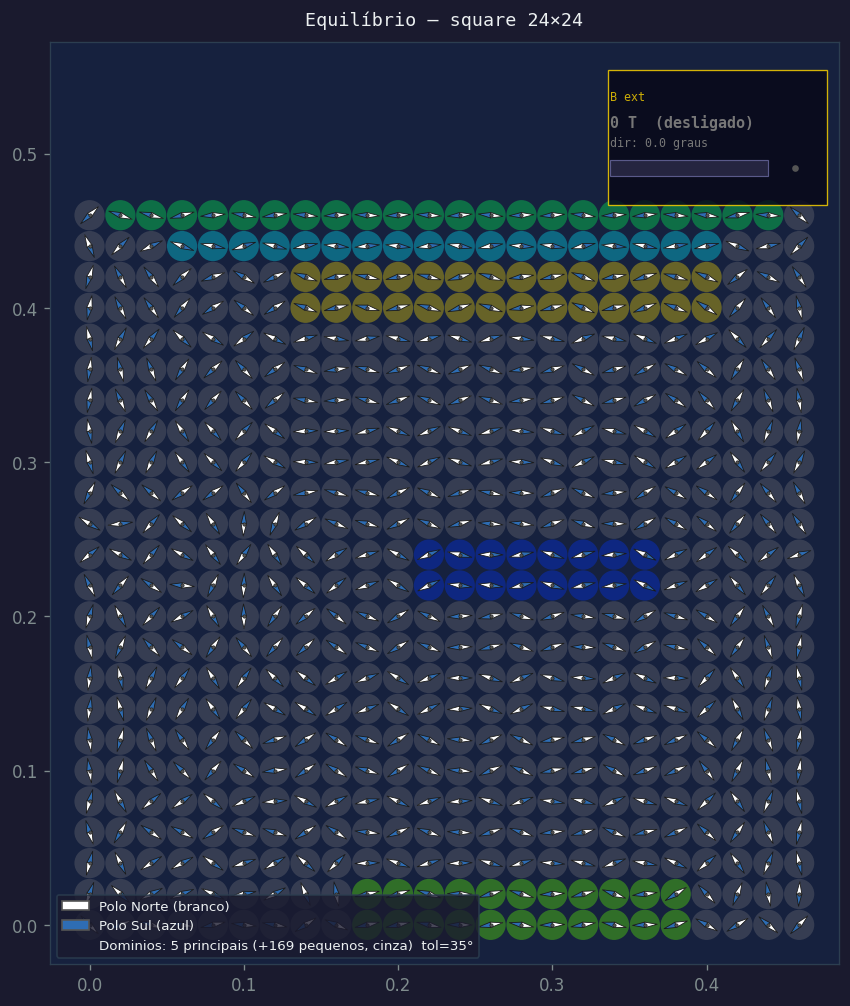
\includegraphics[width=0.72\textwidth]{figs/halo_domains_v3.png}
\caption{Visualização de domínios magnéticos (V38): rede quadrada
$24\times24$ após relaxação longa; os cinco domínios principais recebem
cores distintas e os domínios pequenos aparecem em cinza. A mesma
rotina de rotulagem alimenta a estatística de domínios da campanha
científica.}
\label{fig:dominios}
\end{figure}

\subsection{Fase 6 --- da ferramenta à pesquisa (18/06 e 04/07)}

Com o instrumento maduro, o foco mudou para ciência:

\begin{enumerate}
\item \textbf{Revisão de literatura} (detalhada na
Seção~\ref{sec:pesquisa}) identificando a lacuna e o desenho de estudo;
\item \textbf{Estratégia de publicação} (revistas ACS, acordo CAPES,
alternativas de alto impacto);
\item \textbf{\code{--make\_images} (V39)}: constatou-se que, mesmo sem
\code{--video}, o programa gerava incondicionalmente 4--5 imagens PNG de
resumo por execução --- custo irrelevante em redes grandes, mas
dominante em redes pequenas usadas em varreduras. O novo parâmetro
suprime toda a geração de imagens preservando os CSVs de dados, com
ganho medido de $\sim 3\times$ em execuções pequenas (2{,}03~s $\to$
0{,}65~s em rede $8\times8$);
\item \textbf{Infraestrutura de campanha}: os scripts
\code{damping\_sweep.py} (orquestração da varredura
amortecimento~$\times$~semente~$\times$~geometria, chamando o simulador
programaticamente) e \code{damping\_sweep\_analysis.py} (análise
estatística completa), ambos validados ponta a ponta
(Seção~\ref{sec:campanha});
\item \textbf{Otimizações de desempenho implementadas (04/07)}: o tensor
dipolar pré-computado (\textbf{V40}) e a paralelização da campanha com
\emph{manifest} incremental e retomada (\code{damping\_sweep} V02) ---
detalhes e medições na Seção~\ref{sec:melhorias}. Ganho medido da V40:
\textbf{35--45$\times$} por rodada, reduzindo a campanha completa de
$\sim$7--8~h para $\sim$15~min em um único núcleo;
\item \textbf{Novos protocolos de campo e refinamentos (V41--V45)}:
histerese com espaçamento log-simétrico; pulso com temporização
explícita ($\Delta t$ + $t_{\mathrm{pulse}}$ + equilíbrio por torque);
modos degrau \code{step\_pos}/\code{step\_neg}; flag
\code{--t\_sim\_full} (execução até o fim, sem parada antecipada); halos
também na figura de comparação (V43); painel de progresso vivo de duas
linhas (V44); e o vídeo de histerese com painel duplo --- agulhas e
curva $M\times H$ evoluindo lado a lado (V45). Todos com os modos
legados validados bit-idênticos.
\end{enumerate}

% ======================================================================
\section{Registro de versões}
% ======================================================================

\begin{table}[h]
\centering
\small
\caption{Registro de versões do \code{compass\_sim}. As versões V1--V19
antecedem o registro formal e foram consolidadas retroativamente; a
partir de V20 cada alteração gera uma nova versão numerada.}
\label{tab:versoes}
\begin{tabular}{@{}lp{11.5cm}@{}}
\toprule
\textbf{Versão} & \textbf{Conteúdo principal} \\
\midrule
V1--V19 & Núcleo do simulador: dinâmica dipolar inercial (SI), três
geometrias, campo externo, vídeo MP4, modos de campo
(estático/pulso/histerese/senoidal), exportação CSV, PBC, correções da
honeycomb e da semântica de \code{t\_sim}. \\
V20 & Marco do registro formal de versões. \\
V21--V24 & Refinamento do modo pulso (critério de platô de $S$);
indicadores de tela reposicionados (campo no topo direito, margem
superior dedicada). \\
V25--V28 & Suporte a GPU via CuPy; flag \code{--gpu}; investigação de
utilização; instrumentação de desempenho (throughput, ms/passo). \\
V29--V33 & PBC com imagens da estrutura no campo dipolar (padrão 1
cópia); barra de progresso; momento de inércia automático da geometria
real (aço \SI{0.4}{mm}); Ctrl+C aborta imediatamente / Ctrl+I salva e
sai (código 130). \\
V34 & Consolidação e correções da vetorização GPU do laço de torques. \\
V35 & Otimização da renderização matplotlib por coleções vetorizadas:
ganho de 17--30$\times$; validação bit-a-bit de geometria e física. \\
V36 & Parâmetro \code{--progress\_bar} \{0,1\}. \\
V37 & Momento magnético automático ($m = M_s V$, aço saturado);
correção da regressão de status com \code{--progress\_bar 0}. \\
V38 & Visualização de domínios magnéticos: \code{--halo\_mode domains},
\code{--domain\_tol}; rotulagem por \emph{union--find}; domínios pequenos
em cinza. \\
V39 & Parâmetro \code{--make\_images} \{0,1\}: suprime toda a geração
de PNG preservando CSVs; ganho $\sim 3\times$ em redes pequenas. \\
V40 & Tensor de interação dipolar pré-computado: passos por produto
matriz--vetor (BLAS/cuBLAS); ganho medido de \textbf{35--45$\times$};
validação ao \emph{epsilon} de máquina; proteção de memória com
\emph{fallback} automático. \\
V41 & Novos protocolos de campo: histerese com espaçamento
log-simétrico (\code{--hyst\_spacing log}, amostragem $\sim$15$\times$
mais fina perto de $B{=}0$ para $k{=}5$); pulso com temporização
explícita (\code{--field\_delay}, \code{--t\_pulse}) e critério de
equilíbrio por torque (\code{--torque\_tol}); modos degrau
\code{step\_pos}/\code{step\_neg}. Modos legados bit-idênticos à V40. \\
V42 & Parâmetro \code{--t\_sim\_full} \{0,1\}: com 1, a simulação roda
até o fim de \code{t\_sim}, desativando todas as paradas antecipadas por
critério físico ($S{=}1{,}00$, repouso, equilíbrio por torque) --- útil
para séries temporais de comprimento uniforme em varreduras. Ctrl+I e
Ctrl+C permanecem ativos; padrão (0) bit-idêntico à V41. \\
V43 & Correção reportada pelo usuário: a figura de comparação
(\code{compass\_comparison.png}) não desenhava halo algum (em nenhum
modo) --- os domínios apareciam apenas em \code{compass\_initial.png},
\code{compass\_equilibrium.png} e nos vídeos. A lógica de halos foi
extraída para \code{draw\_halos\_batch()} (reutilizável) e aplicada aos
dois painéis da comparação, com a contagem de domínios no título de
cada painel no modo \code{domains}. Corrigido também o supertítulo da
comparação, que exibia ``B\_ext=0.00'' para campos em mT (formatação
\code{\%.2f} sobre valores pequenos). Figuras de \code{plot\_state}
pixel-idênticas e física bit-idêntica à V42. \\
V44 & Painel de progresso vivo de 2 linhas: barra e status periódico
reescritos em cima de si mesmos (códigos ANSI com invariante de cursor),
eliminando o empilhamento de linhas no terminal --- causado pelo status
de 2~s que fechava a barra com \emph{newline} a cada ciclo. Detecção de
TTY: em saída redirecionada (log/pipe) mantém o comportamento de log
sem códigos de escape. Validado com emulador de terminal
(\code{pyte}): tela final com exatamente 1 linha de barra + 1 de
status; mensagens intercaladas (transições de fase) limpas; física
bit-idêntica. \\
V45 & Vídeo do modo histerese com painel duplo: agulhas à esquerda e
curva $M\times H$ traçada em tempo real à direita (ponto atual
destacado), permitindo acompanhar visualmente a varredura do campo.
Demais modos de vídeo inalterados; física bit-idêntica.
\emph{(Versão atual.)} \\
\midrule
\multicolumn{2}{@{}l}{\emph{Scripts satélites (registro de versões
próprio):}} \\
--- & \code{damping\_sweep} V01: orquestração da campanha
damping~$\times$~seed~$\times$~geometria. \\
--- & \code{damping\_sweep} V02: execução paralela
(\code{--n\_workers}), \emph{manifest} incremental e retomada
(\code{--resume}). \\
--- & \code{damping\_sweep\_analysis.py}: métricas de laço, detecção de
avalanches, ajuste MLE de lei de potência, gráficos. \\
\bottomrule
\end{tabular}
\end{table}

% ======================================================================
\section{Estratégia de pesquisa e publicação}
\label{sec:pesquisa}
% ======================================================================

\subsection{A lacuna na literatura}

A revisão cobriu três frentes. \textbf{(i)}~Redes de agulhas de bússola
clássicas: o trabalho fundador (rede quadrada $22\times22$, Phys.\ Rev.\
B \textbf{58}, 9238, 1998~\cite{prb1998}) usa Monte Carlo de equilíbrio
com campo aleatório imitando ruído térmico --- não dinâmica newtoniana.
\textbf{(ii)}~Dipolos clássicos em redes
honeycomb/kagomé/triangulares (2012--2025): métodos de
Luttinger--Tisza, minimização de energia, ondas de spin e Monte Carlo
com \emph{parallel tempering} --- todos focados em estados fundamentais
e transições térmicas de \emph{equilíbrio}. \textbf{(iii)}~\emph{Artificial
spin ice}~\cite{nisoli2013}: estuda dinâmica temporal real, mas via
macrospins discretos (tipo Ising) ou dados experimentais (MOKE/MFM) ---
quase nunca com dinâmica angular contínua e inércia mecânica explícita.

A pergunta ``como o amortecimento controla histerese e avalanches'' é
ativa e publicável em campos adjacentes --- está estabelecido que os
regimes sub e sobreamortecido formam classes de universalidade
distintas em sistemas de curto alcance ou campo médio~\cite{dahmen2011}
--- mas nunca foi respondida para acoplamento dipolar completo
(longo alcance, anisotrópico) com geometria espacial real. Essa é a
lacuna que o projeto ocupa.

\subsection{Desenho do estudo e critério de decisão}

O estudo central varre o amortecimento por $\sim 2{,}5$ ordens de
grandeza em $Q$ (de $Q \approx 15$, subamortecido, a $Q \approx 0{,}05$,
sobreamortecido), com múltiplas sementes de ruído inicial, nas três
geometrias, medindo: área do laço de histerese, campo coercivo,
remanência, estatística de avalanches (expoente $\tau$ da lei de
potência $P(s) \sim s^{-\tau}$, ajustado por máxima verossimilhança com
o método de Clauset--Shalizi--Newman~\cite{clauset2009}) e distribuição
de tamanhos de domínio na relaxação livre.

O critério de decisão foi definido \emph{a priori}:
\begin{itemize}
\item \textbf{Resultado A (incremental, sólido)}: $\tau$ aproximadamente
constante com $Q$ (apenas escalas/cortes mudam) --- consistente com a
fenomenologia conhecida; publicável nas revistas-alvo padrão;
\item \textbf{Resultado B (surpreendente)}: $\tau$ variando
sistematicamente com $Q$, ou diferença qualitativa entre geometrias ---
assinatura de quebra de universalidade pelo acoplamento dipolar
anisotrópico de longo alcance; justificaria tentar PRL ou similar.
\end{itemize}

\subsection{Revistas-alvo e financiamento de APC}

\begin{itemize}
\item \textbf{Acordo CAPES--ACS}: confirmado que o acordo transformativo
\emph{Read \& Publish} da CAPES cobre \textbf{100\% do APC em qualquer
periódico da ACS} (licença CC~BY) para autores correspondentes de
instituições do consórcio, com elegibilidade verificada na submissão via
ORCID --- removendo o custo como fator de decisão;
\item \textbf{Alvo primário}: \emph{ACS Materials Au} (IF~6{,}5, Q2) ---
maior impacto entre as opções totalmente \emph{open access}; requer
enquadrar o trabalho como modelo para \emph{artificial spin ice} e
nanoímãs em arranjo, o que foi incorporado ao desenho da introdução;
\item \textbf{Alvo reserva}: \emph{ACS Physical Chemistry Au} (IF~4{,}3,
Q2) --- escopo explicitamente inclui matéria condensada; encaixe mais
seguro;
\item \textbf{Alternativas de alto impacto}: \emph{Physical Review
Letters} está \emph{fora} do acordo CAPES (a APS não é editora
conveniada); \emph{Nature Communications}, por ser \emph{gold OA}, é
excluída dos acordos \emph{Read \& Publish} (APC $\sim$ USD~6.190 por
fora). Ambas só se justificam se o resultado for tipo B;
\item \textbf{Outras editoras CAPES} (Springer Nature $\sim$1.750
títulos híbridos, Elsevier $\sim$160, Wiley, IEEE, RSP, ACM): revisão
parcial não encontrou, até a letra~H da lista Springer, título com
encaixe superior aos alvos ACS; candidatos naturais da Elsevier
(\emph{Physica A}, \emph{JMMM}) aguardam verificação na lista de
elegíveis.
\end{itemize}

% ======================================================================
\section{Infraestrutura de campanha e estudo-piloto}
\label{sec:campanha}
% ======================================================================

\subsection{Os dois scripts}

\textbf{\code{damping\_sweep.py}} orquestra a campanha chamando o
simulador programaticamente (sem tocar no código-fonte): constrói a
grade de amortecimentos log-espaçada em $Q$ a partir da física real
(inércia e momento derivados da geometria), executa a Etapa~1
(histerese) e a Etapa~2 (relaxação livre com estatística de domínios)
para cada combinação geometria~$\times$~$Q$~$\times$~semente, e salva
CSVs por rodada, metadados JSON (incluindo $Q$, $\omega_0$,
$B_{\mathrm{ref}}$, distribuição de domínios) e um \code{manifest.csv}
consolidado.

\textbf{\code{damping\_sweep\_analysis.py}} lê o \code{manifest.csv} e
produz: área do laço (integral de linha fechada), coercividade e
remanência (interpolação nos cruzamentos de zero); detecção de
avalanches em $dM/dB$ dentro de cada segmento monotônico da rampa
(limiar robusto de $4\times$MAD); ajuste de lei de potência por MLE com
seleção de $x_{\min}$ por distância KS~\cite{clauset2009} ---
\emph{agregando as avalanches de todas as sementes} de cada ponto
$(geometria, Q)$ antes do ajuste, decisão metodológica necessária para
estatística confiável; e os gráficos finais, incluindo o teste central
$\tau(Q)$ por geometria.

Validações realizadas: área contra laço retangular exato; $B_c$/$M_r$
contra laço sintético com valores conhecidos; detecção de avalanches
contra degraus injetados (recuperação de tamanhos com erro
$\sim$1\%); MLE contra amostra sintética com $\tau = 2{,}5$ exato
(recuperado $2{,}516 \pm 0{,}021$), pelos dois caminhos de código
(pacote \code{powerlaw}, com correção de um bug real da versão
instalada, e implementação própria de reserva --- resultados idênticos).

\subsection{Resultados do estudo-piloto}

Um piloto reduzido (rede $14\times14 = 196$ agulhas, 5 valores de $Q$,
3 sementes, 3 geometrias, ciclo encurtado) validou o pipeline completo
e já exibe o sinal central procurado
(Figura~\ref{fig:tau} e Tabela~\ref{tab:piloto}): o expoente $\tau$
\textbf{cresce sistematicamente com $Q$} nas três geometrias --- de
$\tau \approx 1{,}2$--$1{,}3$ no \emph{crossover} ($Q \approx 0{,}87$)
a $\tau \approx 1{,}7$--$1{,}8$ no regime subamortecido ($Q = 15$). Nos
dois $Q$ mais sobreamortecidos o ciclo encurtado do piloto não gera
avalanches suficientes para ajuste (comportamento correto do pipeline:
reporta indisponibilidade em vez de número espúrio).

\begin{table}[h]
\centering
\small
\caption{Piloto: expoente de avalanche $\tau$ (MLE, avalanches agregadas
entre 3 sementes) por geometria e fator de qualidade. ``---'' indica
estatística insuficiente ($n_{\mathrm{cauda}} < $ mínimo) no ciclo
encurtado do piloto.}
\label{tab:piloto}
\begin{tabular}{@{}lccc@{}}
\toprule
$Q$ & quadrada & triangular & honeycomb \\
\midrule
15{,}0  & $1{,}81 \pm 0{,}15$ & $1{,}69 \pm 0{,}13$ & $1{,}73 \pm 0{,}15$ \\
3{,}60  & $1{,}62 \pm 0{,}10$ & $1{,}51 \pm 0{,}08$ & $1{,}60 \pm 0{,}12$ \\
0{,}866 & $1{,}19 \pm 0{,}04$ & $1{,}29 \pm 0{,}06$ & --- \\
0{,}208 & --- & --- & --- \\
0{,}050 & --- & --- & --- \\
\bottomrule
\end{tabular}
\end{table}

\begin{figure}[t]
\centering

\includegraphics[width=0.8\textwidth]{figs/tau_vs_Q.png}
\caption{Teste central do estudo (piloto): expoente da lei de potência
de avalanches $\tau$ em função do fator de qualidade $Q$, por geometria.
O crescimento sistemático de $\tau$ com $Q$ --- se confirmado na
campanha completa com estatística adequada --- é a assinatura candidata
de dependência da classe de universalidade com o regime de
amortecimento sob acoplamento dipolar.}
\label{fig:tau}
\end{figure}

\begin{figure}[t]
\centering

\includegraphics[width=0.75\textwidth]{figs/area_vs_Q.png}
\caption{Piloto: área do laço de histerese em função de $Q$, por
geometria. A área cresce monotonicamente ao entrar no regime
sobreamortecido (mais dissipação por ciclo), com as três geometrias
qualitativamente semelhantes nesta métrica --- ao contrário do tamanho
de domínio, em que a rede triangular exibe comportamento
não-monotônico a investigar.}
\label{fig:area}
\end{figure}

Dois achados secundários do piloto merecem registro: (i)~a área do laço
e o campo coercivo crescem monotonicamente ao entrar no regime
sobreamortecido (Figura~\ref{fig:area}); (ii)~o tamanho médio de domínio
na rede \emph{triangular} exibe não-monotonicidade com $Q$ que não
aparece nas outras geometrias --- exatamente o tipo de interação
frustração~$\times$~inércia apontada no desenho do estudo como candidata
a resultado tipo~B. Ambos exigem a campanha completa para confirmação.

\subsection{Campanha completa (pronta para execução)}

Parâmetros definidos: rede $30\times30$ (900 agulhas), 8 valores de $Q$
log-espaçados em $[0{,}05;\,15]$, 5 sementes, 3 geometrias
$\Rightarrow$ 120 rodadas de histerese + 120 de relaxação. Custo com o
código V39: $\sim$2--2{,}5~min por rodada ($\approx$~7--8~h de campanha
serial). \textbf{Com a otimização V40} (tensor pré-computado,
Seção~\ref{sec:melhorias}): $\sim$3{,}3--3{,}4~s por rodada
$\Rightarrow$ \textbf{$\sim$15~min de campanha serial em um único
núcleo}, e alguns minutos com \code{--n\_workers} no servidor
\code{jps@mumax} --- sem necessidade de GPU.

% ======================================================================
\section{Roteiro passo a passo dos estudos propostos}
\label{sec:roteiro}
% ======================================================================

Esta seção detalha, em formato operacional, os quatro estudos
identificados como candidatos a publicação, do central aos satélites.
Para cada um: a pergunta, os passos de simulação, a análise, o resultado
esperado e o destino editorial. Todos usam exclusivamente capacidades já
implementadas (V39 + scripts de campanha), salvo onde indicado.

\subsection{Estudo 1 (central): amortecimento como parâmetro de
controle de histerese e avalanches}

\textbf{Pergunta.} O fator de qualidade $Q$ controla a classe de
universalidade das avalanches e a forma do laço de histerese sob
acoplamento dipolar completo? A resposta depende da geometria?

\begin{enumerate}
\item \textbf{Calibração} ($\sim$30~min): agulha isolada em modo pulso;
ajustar o envelope do decaimento livre e validar que o $Q$ medido bate
com $Q = \omega_0 I / b$. Garante que a grade de amortecimentos cobre de
fato os dois regimes;
\item \textbf{Campanha de histerese}: rede $30\times30$; 8 valores de
$Q$ log-espaçados em $[0{,}05;\,15]$; 5 sementes; 3 geometrias; ciclo de
5 rampas com $B_{\max} = 8\,B_{\mathrm{ref}}$ e duração $\propto T_0$
(120 rodadas, $\sim$4{,}5~h em CPU serial);
\item \textbf{Campanha de relaxação}: mesmas combinações com $B = 0$,
partindo do mesmo ruído, até platô de $S$; estatística de domínios no
estado final (120 rodadas, $\sim$3~h);
\item \textbf{Análise} (\code{damping\_sweep\_analysis.py}): área,
$B_c$ e $M_r$ vs.\ $Q$ por geometria; $\tau(Q)$ por MLE com avalanches
agregadas entre sementes; tamanho/número de domínios vs.\ $Q$;
\item \textbf{Robustez} (obrigatória antes de conclusões): convergência
em $\Delta t$ nos extremos de $Q$; tamanhos $N = 20$ e $40$ no ponto
$Q \approx 1$; comparação com/sem PBC;
\item \textbf{Decisão e redação}: critério A/B da
Seção~\ref{sec:pesquisa}; enquadramento ``modelo para \emph{artificial
spin ice} / nanoímãs em arranjo'' na introdução.
\end{enumerate}

\textbf{Resultado esperado.} O piloto sugere $\tau$ crescente com $Q$
nas três geometrias --- se confirmado com estatística plena e sobrevivendo
aos diagnósticos de robustez, é candidato a resultado tipo~B.
\textbf{Destino:} ACS Materials Au (resultado A) ou tentativa em PRL
(resultado B), com ACS Physical Chemistry Au de reserva.

\subsection{Estudo 2 (satélite): frustração geométrica e cinética de
formação de domínios}

\textbf{Pergunta.} A frustração geométrica (triangular $>$ honeycomb $>$
quadrada) acelera ou retarda o engrossamento (\emph{coarsening}) dos
domínios? A não-monotonicidade do tamanho de domínio com $Q$ vista no
piloto da rede triangular é real?

\begin{enumerate}
\item Relaxação livre longa ($B = 0$) nas três geometrias, mesmas
sementes, para 3--4 valores de $Q$ representativos;
\item Registrar $S(t)$ e rotular domínios em instantes intermediários
--- \emph{requer instrumentação pequena}: hoje a estatística de domínios
é calculada apenas no estado final; adicionar \emph{snapshots} periódicos
da rotulagem ao longo da trajetória;
\item Extrair o tempo até o platô de $S$ e a lei de crescimento do
tamanho característico de domínio $L(t) \sim t^{n}$, comparando o
expoente $n$ entre geometrias e regimes de amortecimento.
\end{enumerate}

\textbf{Destino:} pode compor o artigo central (seção de domínios) ou,
se a interação frustração~$\times$~inércia for rica, artigo próprio em
ACS Physical Chemistry Au. Custo computacional baixo (sem rampas de
campo).

\subsection{Estudo 3 (satélite): memória do \emph{director} após pulso}

\textbf{Pergunta.} Após um pulso de campo saturante, o \emph{director}
(direção preferencial emergente, conceito do trabalho de
1998~\cite{prb1998}) que se forma na relaxação guarda memória da direção
do pulso, ou é apagado e redeterminado pelo ruído inicial? Monte Carlo
de equilíbrio não pode responder isso --- exige trajetória temporal
real.

\begin{enumerate}
\item Modo pulso com direção $\varphi$ do campo varrida (por exemplo,
$0^\circ$ a $90^\circ$ em passos de $15^\circ$), várias sementes,
2--3 valores de $Q$;
\item Medir a direção do \emph{director} final (orientação média dos
domínios principais) em função de $\varphi$;
\item Quantificar a correlação direcional
$\langle \cos 2(\theta_{\mathrm{dir}} - \varphi) \rangle$ e sua
dependência com $Q$ --- a hipótese interessante é que a memória seja
mais forte no regime sobreamortecido (sem oscilações que ``sacodem'' o
sistema para fora do vale selecionado pelo pulso).
\end{enumerate}

\textbf{Destino:} conecta-se à literatura recente de \emph{clocked
dynamics} e treinamento em \emph{artificial spin ice}; bom candidato a
segundo artigo. Custo moderado.

\subsection{Estudo 4 (satélite): condições de contorno e tamanho finito
na escala de domínios}

\textbf{Pergunta.} Quanto a borda livre distorce a estatística de
domínios e avalanches em relação ao limite periódico? Sistemas dipolares
de longo alcance são notoriamente sensíveis à forma da amostra; a
resposta é metodologicamente útil para toda a comunidade que simula
essas redes sem PBC.

\begin{enumerate}
\item Varrer $N \in \{14, 20, 30, 40\}$ com e sem PBC, em $Q \approx 1$
e nos dois extremos;
\item Repetir as análises de domínio e avalanche; extrapolar a escala
característica de domínio com $1/N$;
\item Quantificar o desvio sistemático borda-livre vs.\ periódico.
\end{enumerate}

\textbf{Destino:} apêndice/seção de métodos do artigo central, ou nota
metodológica independente. O ponto $N = 40$ sem otimizações é caro
($\mathcal{O}(K^2)$ com $K = 1600$) --- este estudo é o principal
motivador da otimização de desempenho proposta na
Seção~\ref{sec:melhorias}.

% ======================================================================
\section{Melhorias propostas para o código}
\label{sec:melhorias}
% ======================================================================

Análise do código na versão V39 identificou as seguintes oportunidades,
ordenadas por impacto estimado. Nenhuma é bloqueante para o Estudo~1,
que já é viável como está; as de desempenho tornam os Estudos~2--4
substancialmente mais baratos.

\subsection{Desempenho}

\begin{enumerate}
\item \textbf{Pré-computação do tensor de interação dipolar ---
IMPLEMENTADA (V40, 04/07).} As posições das agulhas são fixas --- apenas
os ângulos evoluem --- mas até a V39 as matrizes $K \times K$ de
geometria (deslocamentos, distâncias, potências de $r$, máscaras de
\emph{cutoff} e a soma sobre imagens PBC) eram reconstruídas a cada
passo de integração. Como o campo dipolar é \emph{linear} nos momentos
$(m_x, m_y)$, toda a geometria foi condensada, uma única vez antes do
laço, em três matrizes constantes $A_{xx}, A_{xy}, A_{yy}$
($A_{yx} = A_{xy}$; imagens periódicas já somadas), reduzindo cada passo
a produtos matriz--vetor via BLAS/cuBLAS.

\emph{Validação} (três níveis): torques do tensor vs.\ método por passo
idênticos ao \emph{epsilon} de máquina (erro relativo máximo
$3 \times 10^{-16}$, nas 3 geometrias, com e sem PBC); trajetória
completa de histerese com 172 passos com $t$ e $B$ bit-idênticos à V39 e
$M$, $S$ concordando em $5 \times 10^{-12}$ (acúmulo esperado de
reassociação de ponto flutuante); os 4 modos de campo e o comportamento
de \mbox{Ctrl+C} (código 130) preservados.

\emph{Resultado medido} (rede $30\times30$, mesmos parâmetros do
\emph{baseline}): de 117{,}8~s / 148{,}0~s por rodada de histerese para
\textbf{3{,}4~s / 3{,}3~s} --- ganho de \textbf{35--45$\times$}, acima
da estimativa inicial de 5--20$\times$. O tensor ocupa apenas 19~MB para
$K = 900$. Proteção de memória embutida: acima de 4~GB estimados
(K~$\gtrsim$~13.000), o código informa e cai automaticamente para o
método por passo. A campanha completa de $\sim$7--8~h passou a
$\sim$15~min seriais;
\item \textbf{Paralelização da campanha --- IMPLEMENTADA
(\code{damping\_sweep} V02, 04/07).} Três recursos: \code{--n\_workers~N}
executa rodadas em processos independentes (cada worker em diretório de
trabalho próprio, evitando colisão dos arquivos incidentais gravados
pelo simulador); \emph{manifest} \textbf{incremental}, atualizado após
cada rodada concluída (a versão anterior só o escrevia ao final --- uma
interrupção perdia todo o registro, vulnerabilidade que chegou a se
manifestar durante os testes); e \code{--resume~1}, que retoma campanha
interrompida pulando rodadas já registradas.

\emph{Validação}: execução paralela com 4 \emph{workers} produz CSVs
bit-idênticos aos da execução serial; retomada total (``nada a fazer'')
e parcial (interrupção simulada) funcionam; o script de análise lê o
\emph{manifest} da V02 sem alteração. O ganho de tempo é $\sim$linear no
número de núcleos --- não mensurável no ambiente de desenvolvimento
(1 núcleo), a confirmar no servidor;
\item \textbf{Precisão simples opcional na GPU (proposta).}
\code{float32} dobra o \emph{throughput} de memória; para estatística de
avalanches deve ser suficiente --- validar contra \code{float64} em um
caso antes de adotar;
\item \textbf{Passo de tempo adaptativo no regime sobreamortecido
(proposta; investigar com cautela).} Com $Q \ll 1$ a dinâmica é lenta e
o $\Delta t$ atrelado a $T_0$ é conservador; um passo maior, limitado
pela escala viscosa, reduziria o custo justamente das rodadas mais
lentas. Exige estudo de convergência dedicado antes de adoção. Com o
ganho da V40, deixou de ser prioridade.
\end{enumerate}

Duas otimizações relevantes já estão implementadas e não devem ser
refeitas: a renderização vetorizada (17--30$\times$, V35) e a
codificação de vídeo por NVENC quando \code{--gpu 1}.

\subsection{Aspecto visual}

\begin{enumerate}
\item \textbf{Modo figura de publicação} (\code{--fig\_style paper}):
fundo branco, paleta segura para daltonismo, exportação vetorial
(PDF/SVG), fontes dimensionadas para coluna de artigo e sem elementos de
HUD (cronômetro, indicador de campo). As figuras atuais (tema escuro,
PNG) são ótimas para tela e vídeo, mas inadequadas para o manuscrito ---
esta é a melhoria visual de maior valor imediato para a publicação;
\item \textbf{Curva $M\times H$ ao vivo no vídeo de histerese ---
IMPLEMENTADA (V45).} O vídeo do modo \code{hysteresis} passou a ter
painel duplo: agulhas à esquerda e a curva $M\times H$ à direita,
traçada em tempo real com o ponto atual destacado, comunicando o
experimento inteiro num único vídeo. Os demais modos de vídeo seguem em
painel único; a física é bit-idêntica (mudança só de renderização);
\item \textbf{Destaque visual de avalanches}: realçar agulhas que
giraram acima de um limiar nos últimos $n$ passos, mostrando a
propagação espacial das avalanches e conectando o vídeo à estatística
do artigo;
\item \textbf{Desenho de paredes de domínio}: traçar as arestas entre
domínios de rótulos distintos (complementa os halos coloridos; leitura
mais limpa em redes grandes);
\item \textbf{Seta da magnetização líquida}: vetor $\vec M$ global
sobreposto à rede, com módulo e direção instantâneos;
\item \textbf{Halo em modo energia}: mapa de calor da energia dipolar
por agulha, revelando frustração local e prováveis núcleos de
avalanche.
\end{enumerate}

% ======================================================================
\section{Próximos passos}
% ======================================================================

\begin{enumerate}
\item Executar a campanha completa no servidor (comando documentado nos
scripts; recomenda-se \code{--quick\_test 1} antes, para validar o
ambiente);
\item Rodar a análise e aplicar o critério A/B ao $\tau(Q)$ com
estatística plena; verificar em particular se a inclinação de $\tau(Q)$
difere entre geometrias e se a não-monotonicidade do domínio triangular
sobrevive;
\item Diagnósticos de robustez antes de qualquer conclusão: convergência
em $\Delta t$ nos extremos de $Q$; efeitos de tamanho finito ($N = 20$ e
$40$ no ponto $Q \approx 1$); comparação com/sem PBC;
\item Decidir a revista pelo resultado (A $\to$ ACS Materials Au /
Physical Chemistry Au; B $\to$ considerar PRL) e iniciar o manuscrito
com o enquadramento ``modelo para \emph{artificial spin ice} e nanoímãs
em arranjo'';
\item Estudos satélites do roteiro original, conforme fôlego: cinética
de formação de domínios por geometria; memória do ``director'' após
pulso; efeito de PBC na escala de domínios.
\end{enumerate}

% ======================================================================
\appendix
\section{Apêndice: parâmetros de linha de comando (V45)}
% ======================================================================

Lista completa dos parâmetros aceitos pelo \code{compass\_sim} na versão
V45, extraída diretamente da interface do programa. Parâmetros marcados
``auto'' são calculados da geometria física real quando omitidos, e
sobrescritos se fornecidos explicitamente.

\begingroup
\small
\setlength{\tabcolsep}{5pt}
\renewcommand{\arraystretch}{1.15}

\begin{longtable}{@{}lll p{7.6cm}@{}}
\caption{Parâmetros de linha de comando do \code{compass\_sim} V39.}
\label{tab:parametros}\\
\toprule
\textbf{Parâmetro} & \textbf{Padrão} & \textbf{Unid.} &
\textbf{Descrição} \\
\midrule
\endfirsthead
\toprule
\textbf{Parâmetro} & \textbf{Padrão} & \textbf{Unid.} &
\textbf{Descrição} \\
\midrule
\endhead
\bottomrule
\endlastfoot
\multicolumn{4}{@{}l}{\emph{Geometria da rede}} \\
\midrule
\code{--N} & 8 & --- & Número de linhas de agulhas. \\
\code{--M} & 8 & --- & Número de colunas de agulhas. \\
\code{--R} & 0{,}025 & m & Raio do círculo que circunscreve cada agulha;
a distância entre centros de vizinhos é $2R$ em todas as geometrias. \\
\code{--needle\_frac} & 0{,}80 & --- & Comprimento da agulha como fração
do diâmetro $2R$ (limitado a 0--0{,}8). \\
\code{--geometry} & square & --- & Tipo de rede: \code{square},
\code{triangular} ou \code{honeycomb}. \\
\midrule
\multicolumn{4}{@{}l}{\emph{Física e simulação}} \\
\midrule
\code{--moment} & auto & A$\cdot$m$^2$ & Momento magnético por agulha.
Se omitido: $m = M_s V$, aço saturado ao longo do eixo maior
(usa \code{--steel\_Bsat} e o volume real). \\
\code{--inertia} & auto & kg$\cdot$m$^2$ & Momento de inércia por
agulha. Se omitido: lâmina de aço real,
$I = \tfrac{1}{12}\,\mathrm{massa}\,(L^2 + \mathrm{larg}^2)$. \\
\code{--needle\_thickness} & $4 \times 10^{-4}$ & m & Espessura da
lâmina de aço, usada nos dois cálculos automáticos. \\
\code{--steel\_density} & 7850 & kg/m$^3$ & Densidade do aço (cálculo
automático da inércia). \\
\code{--steel\_Bsat} & 2{,}0 & T & Densidade de fluxo de saturação do
aço (cálculo automático do momento; $M_s = B_{\mathrm{sat}}/\mu_0$).
Faixa típica: 1{,}6--2{,}2~T. \\
\code{--damping} & $5 \times 10^{-8}$ & N$\cdot$m$\cdot$s/rad &
Coeficiente de amortecimento viscoso $b$. Zero = oscilação perpétua. \\
\code{--t\_sim} & 2{,}0 & s & Tempo físico total simulado (soma dos
$\Delta t$ integrados). \\
\code{--t\_sim\_full} & 0 & --- & 1 = roda até o fim de \code{t\_sim},
desativando as paradas antecipadas por critério físico ($S{=}1{,}00$,
repouso, equilíbrio por torque); Ctrl+I/Ctrl+C continuam ativos. Útil
para séries de comprimento uniforme em varreduras. \\
\code{--field\_mode} & static & --- & \code{static},
\code{hysteresis} (ciclo de 5 rampas), \code{sine}, \code{pulse}
(espera $\to$ pulso $\to$ estabilização), \code{step\_pos} ($B{=}0$ por
\code{field\_delay}, depois mantido) ou \code{step\_neg} (campo desde
$t{=}0$, removido em \code{field\_delay}). \\
\code{--hyst\_spacing} & linear & --- & Espaçamento da rampa de
histerese: \code{linear} ou \code{log} (log-simétrico via sinh ---
$dB/dt$ pequeno perto de $B{=}0$, amostragem fina na região da
coercividade; grande perto de $\pm B_{\max}$). \\
\code{--hyst\_log\_k} & 5{,}0 & --- & Concentração do espaçamento
\code{log}: $k \to 0$ recupera o linear; $k{=}5$ concentra
$\sim$15$\times$ mais pontos perto de $B{=}0$. \\
\code{--field\_delay} & 0{,}0 & s & $\Delta t$ de espera: no
\code{pulse}, tempo com $B{=}0$ antes do pulso; no \code{step\_pos},
antes de ligar; no \code{step\_neg}, tempo com campo ligado antes de
remover. \\
\code{--t\_pulse} & --- & s & Duração do pulso (\code{pulse}). Se
omitido, critério legado: campo até $S \geq 0{,}99$ ou platô de $S$. \\
\code{--torque\_tol} & $10^{-3}$ & --- & Tolerância relativa do critério
de equilíbrio nos modos pulso/degrau: encerra quando $\omega_{\max}$
pequeno \emph{e} $\langle|\tau|\rangle < \mathrm{tol}\cdot\tau_{\mathrm{ref}}$
($\tau_{\mathrm{ref}} = I\omega_0^2$) por 50 passos; 0 desliga o
critério de torque. \\
\code{--field\_freq} & 1{,}0 & Hz & Frequência do campo senoidal
(apenas \code{sine}). \\
\code{--dt\_factor} & 0{,}05 & --- & Fração do período natural $T_0$
usada como passo $\Delta t$ (0{,}02--0{,}10). \\
\code{--noise} & 1{,}5 & rad & Amplitude do ruído angular inicial
($0$ = todas para $+x$; $\pi$ = aleatório total). \\
\code{--seed} & 42 & --- & Semente do gerador aleatório
(reprodutibilidade). \\
\code{--pbc} & 0 & --- & Condições periódicas de contorno (0/1);
com 1, bordas interagem com réplicas pela convenção de imagem mínima. \\
\code{--pbc\_images} & 1 & --- & Réplicas somadas de cada lado em cada
direção quando \code{--pbc 1} (padrão: grade $3\times3$ de células). \\
\code{--gpu} & 0 & --- & Backend GPU via CuPy (0/1), com
\emph{fallback} automático para CPU se indisponível. \\
\code{--progress\_bar} & 1 & --- & Barra de progresso em tempo real
(0/1); desligar em logs redirecionados. \\
\code{--halo\_mode} & order & --- & Coloração dos halos: \code{order}
(alinhamento local) ou \code{domains} (domínios conexos, V38). \\
\code{--domain\_tol} & 15{,}0 & graus & Tolerância angular entre
vizinhos para pertencerem ao mesmo domínio (\code{--halo\_mode
domains}). \\
\midrule
\multicolumn{4}{@{}l}{\emph{Campo externo uniforme}} \\
\midrule
\code{--B\_ext} & 0{,}0 & T & Intensidade do campo externo (ex.:
$50 \times 10^{-6}$ = campo terrestre). \\
\code{--phi\_ext} & 0{,}0 & graus & Direção do campo
(0 = $+x$, 90 = $+y$, anti-horário). \\
\code{--ext\_Bx}, \code{--ext\_By} & --- & T & Componentes explícitas;
sobrescrevem \code{--B\_ext}/\code{--phi\_ext}. \\
\midrule
\multicolumn{4}{@{}l}{\emph{Saída}} \\
\midrule
\code{--video} & --- & --- & Nome-base do vídeo MP4 (ffmpeg); numeração
automática \code{nome0000.mp4}, \code{0001}, \dots \\
\code{--frame\_every} & 5 & passos & Intervalo entre frames salvos. \\
\code{--make\_images} & 1 & --- & 0 = desliga \emph{toda} a geração de
PNG (frames e resumos), mantendo os CSVs de dados (V39). \\
\code{--fps} & 24 & --- & Quadros por segundo do vídeo. \\
\code{--dpi} & 120 & --- & Resolução dos frames (redes $>15\times15$:
usar 150--200). \\
\code{--keep\_frames} & desl. & --- & Mantém a pasta de PNGs
intermediários após o MP4. \\
\code{--csv\_order} & t & --- & Ordem das colunas do CSV: \code{t}
$\to$ $t,B,M,S$; \code{B} $\to$ $B,M,S,t$. \\
\end{longtable}
\endgroup

% ======================================================================
\section{Apêndice: exemplos de uso}
\label{app:exemplos}
% ======================================================================

Receitas de linha de comando para os casos de uso mais frequentes,
verificadas contra a versão V45. Todos os comandos assumem
\code{python3 compass\_simV45.py} como base; a barra invertida final
indica continuação de linha no \emph{shell}.

\subsection*{B.1 --- Execução básica (equilíbrio dipolar)}

Rede quadrada $8\times8$ com todos os padrões (agulha de aço com
momento e inércia calculados automaticamente, sem campo externo):
\begin{verbatim}
python3 compass_simV45.py --N 8 --M 8 --geometry square
\end{verbatim}
Gera as imagens de resumo (estado inicial, equilíbrio, comparação,
parâmetro de ordem) e o CSV \code{compass\_field\_log.csv} no diretório
corrente. Para as outras redes: \code{--geometry triangular} ou
\code{--geometry honeycomb}.

\subsection*{B.2 --- GPU ligada e desligada}

A CPU é o padrão (\code{--gpu 0}). Com a otimização V40, a CPU já
resolve redes médias em segundos; a GPU vale para redes grandes:
\begin{verbatim}
# CPU (padrao) -- rede media
python3 compass_simV45.py --N 30 --M 30 --t_sim 5.0

# GPU (CuPy/RTX 3090) -- rede grande; requer cupy instalado
python3 compass_simV45.py --N 60 --M 60 --t_sim 5.0 --gpu 1
\end{verbatim}
Com \code{--gpu 1}, a codificação do vídeo também usa o
\emph{encoder} de hardware NVENC quando disponível. Se o CuPy não
estiver funcional, o programa avisa e cai para CPU automaticamente.

\subsection*{B.3 --- Vídeo e figuras em boa resolução}

Para redes acima de $15\times15$, usar \code{--dpi} 150--200. Menor
\code{--frame\_every} = animação mais suave (mais frames):
\begin{verbatim}
python3 compass_simV45.py --N 20 --M 20 --t_sim 4.0 \
    --video demo --dpi 180 --fps 30 --frame_every 3
\end{verbatim}
O vídeo recebe numeração automática (\code{demo0000.mp4},
\code{demo0001.mp4}, \dots). Para manter também os PNGs individuais dos
frames após montar o vídeo, acrescentar \code{--keep\_frames}. Para
apenas figuras estáticas em alta resolução (sem vídeo), basta omitir
\code{--video} e usar \code{--dpi 200}.

\subsection*{B.4 --- Varreduras rápidas: sem imagens, sem barra}

Em campanhas com muitas execuções, desligar toda a geração de imagens
(mantém os CSVs de dados) e a barra de progresso:
\begin{verbatim}
python3 compass_simV45.py --N 8 --M 8 --t_sim 1.0 \
    --make_images 0 --progress_bar 0
\end{verbatim}
Ganho de $\sim 3\times$ em redes pequenas, onde a renderização domina o
tempo. Para séries temporais de comprimento \emph{uniforme} entre
rodadas (sem paradas antecipadas por $S{=}1{,}00$, repouso ou
equilíbrio), acrescentar \code{--t\_sim\_full 1} (V42).

\subsection*{B.5 --- Controle do amortecimento (regimes dinâmicos)}

O regime é caracterizado pelo fator de qualidade $Q$, impresso no
cabeçalho de cada execução junto com a classificação
(sub-/super-amortecido). O valor exato de $Q$ depende do campo
dominante (dipolar ou externo); os valores abaixo, com os demais
parâmetros no padrão, ilustram os três regimes:
\begin{verbatim}
# subamortecido (Q >> 1): oscila visivelmente antes de estabilizar
python3 compass_simV45.py --N 10 --M 10 --damping 5e-8 --video sub

# intermediario (Q ~ 1): crossover
python3 compass_simV45.py --N 10 --M 10 --damping 1e-6 --video meio

# sobreamortecido (Q << 1): relaxacao monotona, sem oscilacao
python3 compass_simV45.py --N 10 --M 10 --damping 5e-5 --video sobre
\end{verbatim}
Conferir o $Q$ impresso no cabeçalho e ajustar \code{--damping} até o
regime desejado. \code{--damping 0} desliga a dissipação (oscilação
perpétua).

\subsection*{B.6 --- Tamanho e espaçamento das agulhas}

O raio $R$ do círculo circunscrito define o espaçamento da rede
($r_{nn} = 2R$); \code{--needle\_frac} define o comprimento da agulha
como fração de $2R$; a espessura da lâmina afeta os cálculos
automáticos de inércia e momento:
\begin{verbatim}
# agulhas de 1 cm de raio, ocupando metade do diametro disponivel
python3 compass_simV45.py --N 12 --M 12 --R 0.01 --needle_frac 0.5

# lamina mais fina (0.2 mm): agulha mais leve -> oscila mais rapido
python3 compass_simV45.py --N 12 --M 12 --needle_thickness 2e-4

# sobrescrever os calculos automaticos com valores explicitos
python3 compass_simV45.py --N 12 --M 12 --moment 0.05 --inertia 1e-9
\end{verbatim}

\subsection*{B.7 --- Campo externo: os seis modos}

Um exemplo por modo, cobrindo todo o leque de \code{--field\_mode}. A
amplitude é \code{--B\_ext} e a direção \code{--phi\_ext}.

\medskip\noindent\textbf{(1) static} --- campo constante (ou nulo)
durante toda a simulação:
\begin{verbatim}
python3 compass_simV45.py --N 10 --M 10 --B_ext 1e-3 --phi_ext 45
\end{verbatim}

\noindent\textbf{(2) hysteresis} --- ciclo de 5 rampas
($0 \to +B_{\max} \to 0 \to -B_{\max} \to 0 \to +B_{\max}$). O vídeo
(V45) mostra, lado a lado, as agulhas e a curva $M\times H$ traçada em
tempo real. Espaçamento \code{linear} (padrão) ou \code{log} (amostragem
$\sim$15$\times$ mais fina na região da coercividade):
\begin{verbatim}
# linear, com video de painel duplo (agulhas + curva M x H)
python3 compass_simV45.py --N 20 --M 20 --field_mode hysteresis \
    --B_ext 0.002 --t_sim 10.0 --video hist --dpi 160

# espacamento log-simetrico (fino perto de B=0)
python3 compass_simV45.py --N 20 --M 20 --field_mode hysteresis \
    --hyst_spacing log --hyst_log_k 5 --B_ext 0.002 --t_sim 10.0
\end{verbatim}

\noindent\textbf{(3) sine} --- campo senoidal
$B(t) = B_{\max}\sin(2\pi f t)$; \code{--t\_sim} deve cobrir vários
períodos:
\begin{verbatim}
python3 compass_simV45.py --N 15 --M 15 --field_mode sine \
    --B_ext 0.002 --field_freq 0.5 --t_sim 8.0
\end{verbatim}

\noindent\textbf{(4) pulse} --- espera \code{field\_delay}, aplica por
\code{t\_pulse}, zera e estabiliza (equilíbrio por $\omega$ e torque). Se
\code{--t\_pulse} for omitido, mantém o critério legado (campo até
$S \geq 0{,}99$ ou platô):
\begin{verbatim}
# temporizado: espera 0.2 s -> campo 0.3 s -> zera e estabiliza
python3 compass_simV45.py --N 15 --M 15 --field_mode pulse \
    --field_delay 0.2 --t_pulse 0.3 --B_ext 0.005 --t_sim 6.0

# legado (sem t_pulse): campo ate saturar, depois relaxa
python3 compass_simV45.py --N 15 --M 15 --field_mode pulse \
    --B_ext 0.005 --t_sim 6.0
\end{verbatim}

\noindent\textbf{(5) step\_pos} --- $B{=}0$ por \code{field\_delay},
depois campo ligado e mantido até o fim:
\begin{verbatim}
python3 compass_simV45.py --N 15 --M 15 --field_mode step_pos \
    --field_delay 0.3 --B_ext 0.003 --t_sim 3.0
\end{verbatim}

\noindent\textbf{(6) step\_neg} --- campo desde $t{=}0$, removido em
\code{field\_delay} e mantido em zero até o fim:
\begin{verbatim}
python3 compass_simV45.py --N 15 --M 15 --field_mode step_neg \
    --field_delay 0.3 --B_ext 0.003 --t_sim 3.0
\end{verbatim}

\noindent Em \code{hysteresis} o laço $M(B)$ é exportado em
\code{hysteresis\_loop.csv}; em \code{sine}, em \code{sine\_field.csv}.
Nos modos pulso/degrau, \code{--torque\_tol} controla o critério de
equilíbrio e \code{--t\_sim\_full 1} desativa a parada antecipada
(Apêndice~A).

\subsection*{B.8 --- Visualização de domínios magnéticos}

Cenário de demonstração que produz domínios claros e bem separados
(rede quadrada com pouco ruído inicial e relaxação longa):
\begin{verbatim}
python3 compass_simV45.py --N 24 --M 24 --R 0.01 --noise 0.6 \
    --t_sim 8.0 --damping 3e-6 \
    --halo_mode domains --domain_tol 35 --video dominios --dpi 160
\end{verbatim}
Cada região conexa de agulhas com orientação similar (dentro de
\code{--domain\_tol} graus) recebe uma cor; domínios pequenos aparecem
em cinza. Tolerâncias menores (por exemplo, o padrão $15^\circ$)
fragmentam mais; maiores agregam mais. A partir da V43, os halos
(de domínio ou de ordem) aparecem em \emph{todas} as figuras —
\code{compass\_initial}, \code{compass\_equilibrium}, os frames de
vídeo e também a \code{compass\_comparison}, cujos painéis mostram a
contagem de domínios de cada estado no título.

\subsection*{B.9 --- Condições periódicas de contorno e
reprodutibilidade}

\begin{verbatim}
# rede tratada como estrutura periodica infinita (1 replica por lado)
python3 compass_simV45.py --N 16 --M 16 --pbc 1 --pbc_images 1

# reprodutibilidade exata: fixar a semente do ruido inicial
python3 compass_simV45.py --N 10 --M 10 --seed 123
\end{verbatim}

\subsection*{B.10 --- Campanha científica completa (scripts satélites)}

\begin{verbatim}
# validacao rapida do ambiente (segundos)
python3 damping_sweepV02.py --out_dir resultados --quick_test 1

# campanha completa do Estudo 1, paralela em 8 nucleos
python3 damping_sweepV02.py --out_dir resultados \
    --grid_n 30 --n_seeds 5 --n_dampings 8 \
    --Q_min 0.05 --Q_max 15.0 \
    --geometries square,triangular,honeycomb --n_workers 8

# retomar campanha interrompida (pula rodadas ja registradas)
python3 damping_sweepV02.py --out_dir resultados ... --resume 1

# analise: metricas de laco, avalanches, tau(Q), dominios
python3 damping_sweep_analysis.py --sweep_dir resultados \
    --out_dir analise
\end{verbatim}
Evitar combinar \code{--n\_workers} $> 1$ com \code{--use\_gpu 1}
(contenção da GPU entre processos).

% ======================================================================
\section*{Histórico de versões deste relatório}
\addcontentsline{toc}{section}{Histórico de versões deste relatório}
% ======================================================================

\begin{tabular}{@{}lll@{}}
\toprule
\textbf{Versão} & \textbf{Data} & \textbf{Alterações} \\
\midrule
V01 & 04/07/2026 & Versão inicial. \\
V02 & 04/07/2026 & Adicionado o Apêndice~A (parâmetros de linha de
comando da V39). \\
V03 & 04/07/2026 & Adicionadas as Seções~\ref{sec:roteiro} (roteiro
passo a passo dos estudos propostos) e \ref{sec:melhorias} (melhorias
propostas para o código: desempenho e visual). \\
V04 & 04/07/2026 & Documentada a implementação das melhorias de
desempenho 1 e 2 (código V40: tensor pré-computado, 35--45$\times$;
\code{damping\_sweep} V02: paralelização, \emph{manifest} incremental,
retomada), com validações e medições; atualizados os custos da campanha
e o registro de versões. \\
V05 & 04/07/2026 & Adicionado o Apêndice~B (exemplos de uso: GPU,
vídeo/figuras em alta resolução, regimes de amortecimento, geometria das
agulhas, modos de campo, domínios, PBC e campanha completa). \\
V06 & 04/07/2026 & Documentada a V41 do código: histerese com
espaçamento log-simétrico, pulso com temporização explícita
($\Delta t$ + $t_{\mathrm{pulse}}$ + equilíbrio por torque) e modos
degrau \code{step\_pos}/\code{step\_neg}; atualizados a Seção~2, o
registro de versões e os Apêndices A e B. \\
V07 & 04/07/2026 & Documentada a V42 do código: parâmetro
\code{--t\_sim\_full} (execução até o fim de \code{t\_sim}, sem paradas
antecipadas por critério físico). \\
V08 & 04/07/2026 & Documentada a V43 do código: halos (ordem e
domínios) agora também na figura de comparação, com contagem de
domínios por painel; correção da formatação de \code{B\_ext} no
supertítulo da comparação. \\
V09 & 04/07/2026 & Documentada a V44 do código: painel de progresso de
2 linhas (barra + status) atualizado no lugar, com detecção de TTY. \\
V10 & 05/07/2026 & Documentada a V45 (vídeo de histerese com painel
duplo agulhas + $M\times H$). Revisão editorial: Apêndice~B.7
reescrito como referência dos seis modos de campo (sem redundância);
versões dos comandos de exemplo padronizadas para V45; título do
Apêndice~A atualizado; cronologia da Fase~6 estendida até a V45. \\
\bottomrule
\end{tabular}

% ======================================================================
\begin{thebibliography}{9}

\bibitem{dahmen2011}
K.~A. Dahmen, Y.~Ben-Zion, J.~T. Uhl,
\emph{A simple analytic theory for the statistics of avalanches in
sheared granular materials},
Nature Physics \textbf{7}, 554 (2011).

\bibitem{nisoli2013}
C.~Nisoli, R.~Moessner, P.~Schiffer,
\emph{Colloquium: Artificial spin ice: Designing and imaging magnetic
frustration},
Reviews of Modern Physics \textbf{85}, 1473 (2013).

\bibitem{prb1998}
Rede quadrada de agulhas magnetizadas interagentes: propriedades
termodinâmicas via campo aleatório e Monte Carlo,
Physical Review B \textbf{58}, 9238 (1998).

\bibitem{clauset2009}
A.~Clauset, C.~R. Shalizi, M.~E.~J. Newman,
\emph{Power-law distributions in empirical data},
SIAM Review \textbf{51}, 661 (2009).

\end{thebibliography}

\end{document}
